\documentclass[hyperref]{article}
%MS%%%%%%%%%%%%%%%%%%%% Article Format %%%%%%%%%%%%%%%%%
%+++++++++++++++++++++ Usepackage +++++++++++++++%%
\usepackage{graphicx} %% Package for Figure
\usepackage{float} %% Package for Float
\usepackage{amssymb}
\usepackage{amsmath}
\usepackage{mathtools}
\usepackage[thmmarks,amsmath]{ntheorem} %% If amsmath is applied, then amsma is necessary
\usepackage{bm} %% Bold Mathematical Symbols
\usepackage[colorlinks,linkcolor=cyan,citecolor=cyan]{hyperref}
\usepackage{extarrows}
\usepackage[hang,flushmargin]{footmisc} %% Let the footnote not indentation
\usepackage[square,comma,sort&compress,numbers]{natbib} %% Sort of References
\usepackage{mathrsfs} %% Swash letter
\usepackage[font=footnotesize,skip=0pt,textfont=rm,labelfont=rm]{caption,subcaption} 
%% Format of Caption for Tab. and Fig.
\usepackage{booktabs} %% tables with three lines
\usepackage{tocloft}
\usepackage{graphicx}

%\usepackage{algorithm}  
%%\usepackage{algorithmicx}  
%\usepackage{algorithmic}
\usepackage[linesnumbered,boxed,commentsnumbered,ruled]{algorithm2e}

%+++++++++++++++ Proof etc. +++++++++++++++++++++++++%%
{%% Environment of Proof
	\theoremstyle{nonumberplain}
	\theoremheaderfont{\bfseries}
	\theorembodyfont{\normalfont}
	\theoremsymbol{\mbox{$\Box$}}
	\newtheorem{proof}{Proof}
}

\usepackage{theorem}
\newtheorem{theorem}{Theorem}[section]
\newtheorem{lemma}{Lemma}[section]
\newtheorem{definition}{Definition}[section]
\newtheorem{assumption}{Assumption}[section]
\newtheorem{example}{Example}[section]
\newtheorem{corollary}{Corollary}[section]
{%% Environment of Remark
	\theoremheaderfont{\bfseries}
	\theorembodyfont{\normalfont}
	\newtheorem{remark}{Remark}[section]
}
\usepackage{abstract}
\renewcommand{\abstractnamefont}{\Large\bfseries}
%\numberwithin{equation}{section} %% Number of Equation
%++++++++++++++++++++++++++++++++ Page format ++++++++++++++++++++++++++%%
\graphicspath{{figure/}}                                 %% Path of Figures
\usepackage[a4paper]{geometry}                           %% Paper size
\geometry{left=2.5cm,right=2.5cm,top=2.5cm,bottom=2.5cm} %% Margin
\linespread{1.2}      
\usepackage{cite}

% matlab code package
\usepackage{appendix}
\usepackage{listings}%插入代码
\usepackage{color}
\lstset{%代码格式的配置
	extendedchars=false,            % Shutdown no-ASCII compatible
	language=Matlab,                % !!!选择代码的语言
	basicstyle=\footnotesize\tt,    % the size of the fonts that are used for the code
	tabsize=3,                            % sets default tabsize to 3 spaces
	numbers=left,                   % where to put the line-numbers
	numberstyle=\tiny,              % the size of the fonts that are used for the line-numbers
	stepnumber=1,                   % the step between two line-numbers. If it's 1 each line
	% will be numbered
	numbersep=5pt,                  % how far the line-numbers are from the code   %
	keywordstyle=\color[rgb]{0,0,1},                % keywords
	commentstyle=\color[rgb]{0.133,0.545,0.133},    % comments
	stringstyle=\color[rgb]{0.627,0.126,0.941},      % strings
	backgroundcolor=\color{white}, % choose the background color. You must add \usepackage{color}
	showspaces=false,               % show spaces adding particular underscores
	showstringspaces=false,         % underline spaces within strings
	showtabs=false,                 % show tabs within strings adding particular underscores
	frame=single,                   % adds a frame around the code
	captionpos=b,                   % sets the caption-position to bottom
	breaklines=true,                % sets automatic line breaking
	breakatwhitespace=false,        % sets if automatic breaks should only happen at whitespace
	title=\lstname,                 % show the filename of files included with \lstinputlisting;
	% also try caption instead of title
	mathescape=true,escapechar=?    % escape to latex with ?..?
	escapeinside={\%*}{*)},         % if you want to add a comment within your code
	%columns=fixed,                  % nice spacing
	%morestring=[m]',                % strings
	%morekeywords={%,...},%          % if you want to add more keywords to the set
	%    break,case,catch,continue,elseif,else,end,for,function,global,%
	%    if,otherwise,persistent,return,switch,try,while,...},%
}
\usepackage{enumitem}
% \setlength{\parskip}{0.4em}
\usepackage{diagbox}

                                   %% Line Spread
%MS%%%%%%%%%%%%%%%%%%%%%%%%%%%% End Format %%%%%%%%%%%%%%%%%%%%%%%%%%%%%%%%%%

%MS%%%%%%%%%%%%%%%%%%%%%%%%%%%%%%%%%%%%%%%%%%%
%MS                                         %%
%MS        The Main Body begins here        %%
%MS                                         %%
%MS%%%%%%%%%%%%%%%%%%%%%%%%%%%%%%%%%%%%%%%%%%%

%MS++++++++++++++++++++++++++++++ Title +++++++++++++++++++
\title{ME5413 Autonomous Mobile Robotics: \\[0.5cm] Final Project}
\author{\textup{Chen Yihui \ \ \ A0263115N \\ Wang Renjie \ A0263387U \\ Shen Yixiu \ \ \ A0263954U \\ Wang Longfei \ A }}
\begin{document}
	\begin{titlepage}
		\center
		\newcommand{\HRule}{\rule{\linewidth}{0.5mm}}
		\includegraphics[width=8cm]{logo.png}\\[1cm] 
		\quad\\[2cm]
		\textsl{\Large National University of Singapore}\\[0.5cm] 
		\textsl{\large College of Design and Engineering}\\[0.5cm]
		\makeatletter
		\HRule \\[0.4cm]
		{ \huge \bfseries \@title}\\[0.4cm] 
		\HRule \\[2cm]
		\begin{minipage}{0.4\textwidth}
			\begin{flushleft} \large
				\emph{Group 9:}\\
				\@author 
			\end{flushleft}
		\end{minipage}
		~
		\begin{minipage}{0.4\textwidth}
			\begin{flushright} \large
				\emph{Supervisor:} \\
				\textup{Prof. Marcelo H Ang Jr}
			\end{flushright}
		\end{minipage}\\[1cm]
		\makeatother
		{\large \emph{Github repo link: https://github.com/Wang-Theo/ME5413\_Final\_Project}}\\[0.5cm]
		{\large \emph{Email Address: e1010473@u.nus.edu \\	\ \ \ \ \ \ \ \ \ \ \ \ \ \ \ \ \ \ \ \ e1010745@u.nus.edu \\	\ \ \ \ \ \ \ \ \ \ \ \ \ \ \ \ \ \ \ \
		e@u.nus.edu \\	\ \ \ \ \ \ \ \ \ \ \ \ \ \ \ \ \ \ \ \
		e@u.nus.edu }}\\[0.5cm]
		{\large \today}\\[2cm] 
		\vfill 
	\end{titlepage}

\section{Project Description}
\hspace{1.0em}
This is the final project of ME5413 Autonomous Mobile Robotics AY22-23 Semester 2. We are given a mini-factory environment which is shown in Fig.~\ref{fig1} in Gazebo. This environment has 3 accessible areas and 1 inaccessible area.

\begin{figure}[H]
	\centering
	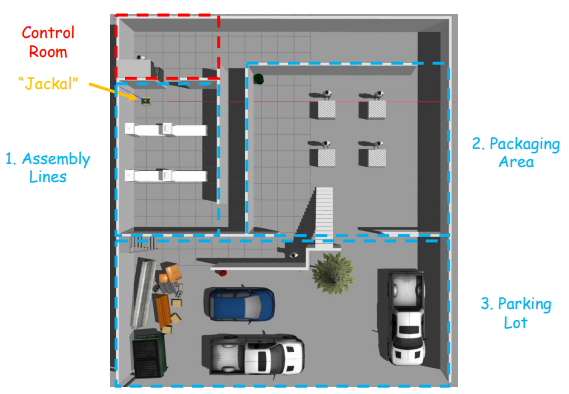
\includegraphics[width=8cm]{map_given.png}
	\caption{Mini-factory environment}
	\label{fig1}
\end{figure}

The aim of the project is to design a robot navigation software stack that can: From the starting point, move to the given pose within each area in sequence:

\begin{itemize}[itemsep=3pt,topsep=0pt,parsep=0pt]
	\item Assembly Line 1, 2
	\item Packaging Area 1, 2, 3, 4
	\item Delivery Vehicle 1, 2, 3
\end{itemize}

Thus, the tasks consist of mapping and navigation.

\section{Task 1 Mapping}
\hspace{1.0em}
In this task, we need to choose an algorithm to map the environment and then also evaluate its accuracy. 

Here as we can see from Fig.~\ref{fig1}, there are some complex and special objects like glass wall, stair, debris and tree. For example, the glass cannot be scanned by lidar except the outline border, the stair is a three-dimensional structure and debris are piled up in different sizes etc. 

We realize that 2D SLAM algorithm is not capable to map the features of these special objects. And also considering that visual SLAM obtains too much information, thus the amount of calculations and loads are large. As the environment here is not too complicated and only simple navigation task is required, the use of lidar is the most suitable. 

Thus, we decide to choose FAST-LIO to do the mapping which use the fusion of 3D LiDAR and IMU.

\subsection{Map the Environment with FAST-LIO}
\hspace{1.0em}
FAST-LIO is a computationally efficient and robust Lidar-Imu Odometry method proposed by the MARS Laboratory of the University of Hong Kong. It utilizes tightly coupled, iteratively extended Kalman filters to fuse lidar landmarks with IMU data for robust navigation in fast-motion, noisy or clutterous environments.

In this task, we refer the repo$^{[1]}$ of the FAST-LIO original authors. Our operation process to build the repo can be concluded as:

\begin{itemize}[itemsep=3pt,topsep=0pt,parsep=0pt]
	\item Git clone the \textit{“ME5413\_Final\_Project”} repo given and follow the readme to build it.
	\item Git clone and build FAST-LIO in our own workspace.
	\item Move FAST-LIO into \textit{“ME5413\_Final\_Project/src”} folder as a package in the repo whose name is \textit{“FAST\_LIO\_”}.
	\item Use command \textit{“roslaunch me5413\_world world.launch”} to launch the world and use \textit{“rostopic list”} to find the two topics we need: pointcloud topic \textit{“/mid/points”} for 3D LiDAR and sensor\_msgs/Imu topic \textit{“/imu/data”} for IMU.
	\item Set the LiDAR pointcloud topic name and IMU topic name in \textit{“velodyne.yaml”} in config folder of \textit{“FAST\_LIO\_”} which is shown in \textit{velodyne.yaml} in Appendix.
	\item Create a new launch file \textit{“fast\_lio.launch”} in the launch folder of \textit{“me5413\_world”} package which is shown in \textit{fast\_lio.launch} in Appendix.
	\item Remake the repo using command \textit{“catkin\_make”}.
\end{itemize}

Thus, now we can successfully do the mapping with command \textit{“roslaunch me5413\_world world.launch”} in first terminal and command \textit{“roslaunch me5413\_world fast\_lio.launch”} in second terminal.

However, we found that there are two problems occurring. First one is we need to cut off the ground pointclouds which is shown in Fig.~\ref{fig2}.

\begin{figure}[H]
	\centering
	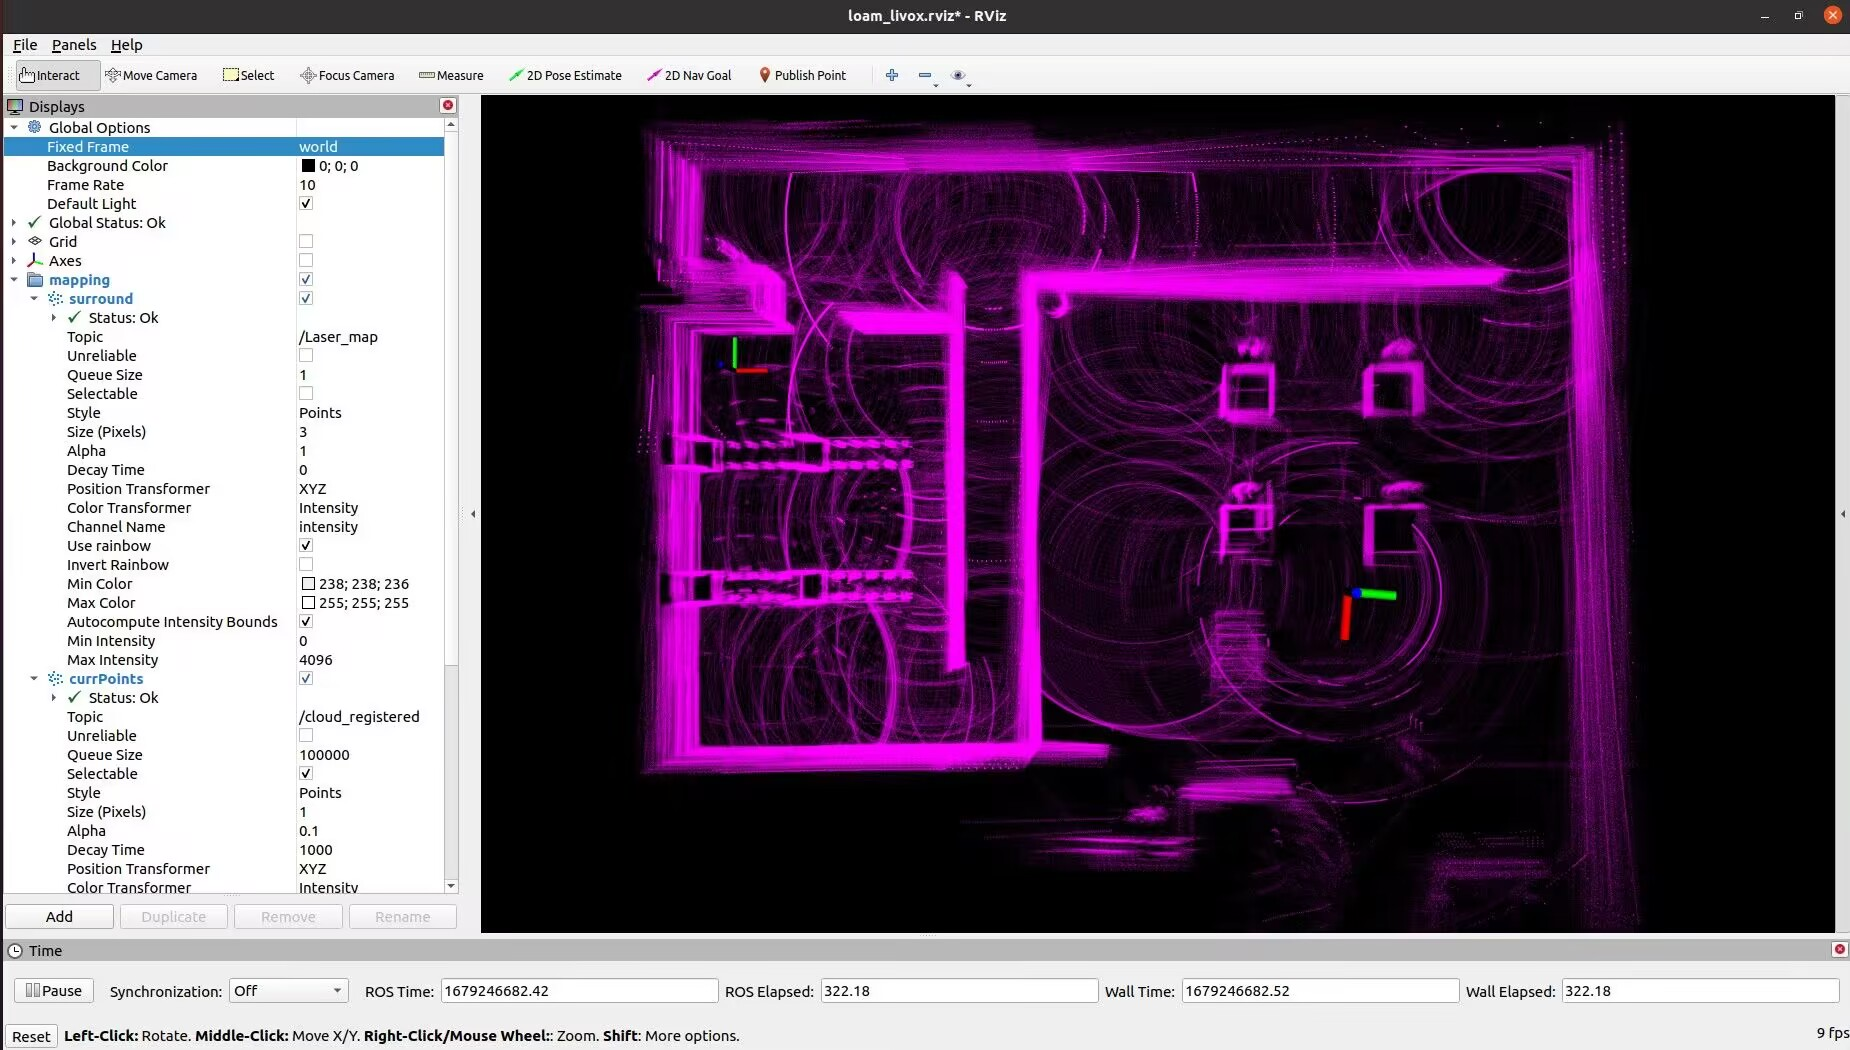
\includegraphics[width=9cm]{problem_ground_truth.jpg}
	\caption{Problem 1: not cut off ground pointclouds}
	\label{fig2}
\end{figure}

The second one is when we turn the Jackal, the pointclouds sometimes fail to coincide with original one, like there will be two sets of pointclouds for one wall in different direction which is shown in Fig.~\ref{fig3}.

\begin{figure}[H]
	\centering
	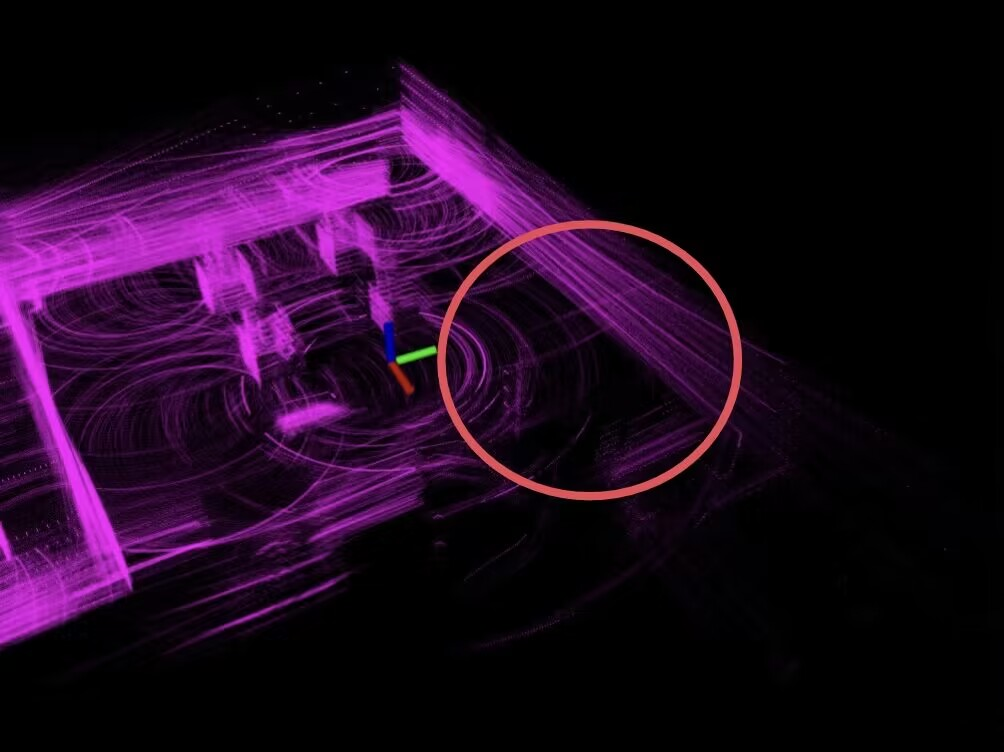
\includegraphics[width=6cm]{problem_fail_coincide.jpg}
	\caption{Problem 2: fail to coincide with original pointclouds}
	\label{fig3}
\end{figure}

To solve the first problem, we add a limit height in $z$ axis for pointclouds in the callback function in \textit{“LaserMapping.cpp”} in \textit{“FAST\_LIO\_”} which is shown in \textit{pointcloud callback function} in \textit{LaserMapping.cpp} in Appendix. This could allow to not publish the ground pointclouds in RViz. And we also filter the ground pointclouds in the result \textit{scans.pcd} file which will be introduced later.

To solve the second problem, we try couple of methods and finally we find that if we increase the 3D LiDAR’s rate from 10Hz to 50 Hz in \textit{“velodyne.yaml”}, the problem will be solved.

Then now if we follow again the process steps introduced, the pointcloud \textit{scans.pcd} file will be saved. But this pointcloud file still have some noise points and ground points need to be filtered. We also need to convert the \textit{pcd} file to a planar grid map which will help do the navigation task.

Thus, we write another package \textit{“pcdtomap”} into \textit{“ME5413\_Final\_Project/src”}. The remaining process are:

\begin{itemize}[itemsep=3pt,topsep=0pt,parsep=0pt]
	\item Create a package named \textit{“pcdtomap”} and write the algorithm with two filter: pass-through filter and radius filter in \textit{“pcdtomap.cpp”}.
\end{itemize}

Notice that pass-through filter here is for filtering the ground pointclouds in $z$ axis and pointclouds too far away in $x$ and $y$ axis, radius filter is for filtering the noise points.

\begin{itemize}[itemsep=3pt,topsep=0pt,parsep=0pt]
	\item Build package structure and write makefile.
	\item Add a launch file \textit{“pcdtomap.launch”} to set the parameters for filters and launch to convert pcd to grid map.
\end{itemize}

Finally, the whole process is done. We can do the mapping task with command:

\begin{itemize}[itemsep=3pt,topsep=0pt,parsep=0pt]
	\item \textit{"roslaunch me5413\_world world.launch”} in first terminal.
	\item \textit{"roslaunch me5413\_world fast\_lio.launch”} in second terminal.
	\item \textit{"roslaunch pcdtomap pcdtomap.launch”} in third terminal.
	\item \textit{"rosrun map\_server map\_saver”} in the forth terminal while in map folder.
\end{itemize}


The RViz, pcd file and grid map result of mapping is shown in Fig.~\ref{fig4}.

\begin{figure}[H]
	\centering
	\begin{minipage}[t]{0.32\textwidth}
		\centering
		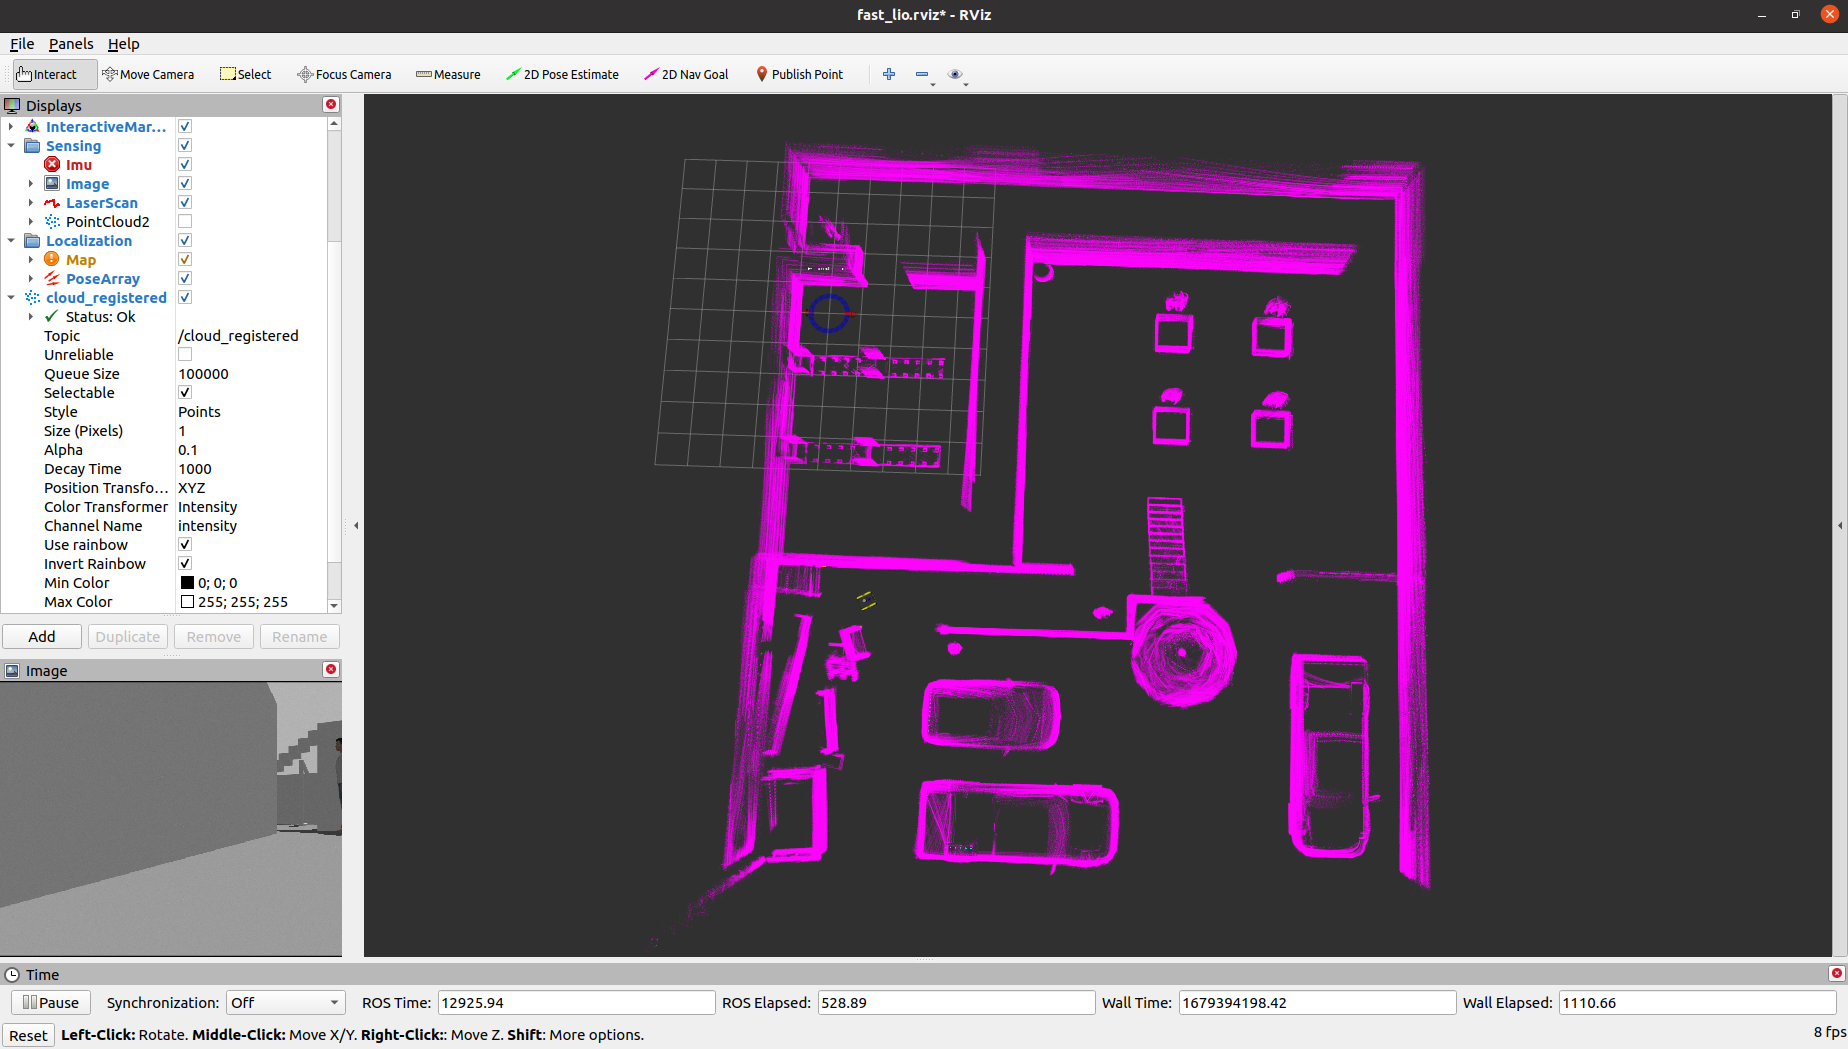
\includegraphics[width=5cm]{RViz_shot.png}
		\subcaption{RViz shot}
		\label{fig4a}
	\end{minipage}
	\begin{minipage}[t]{0.32\textwidth}
		\centering
		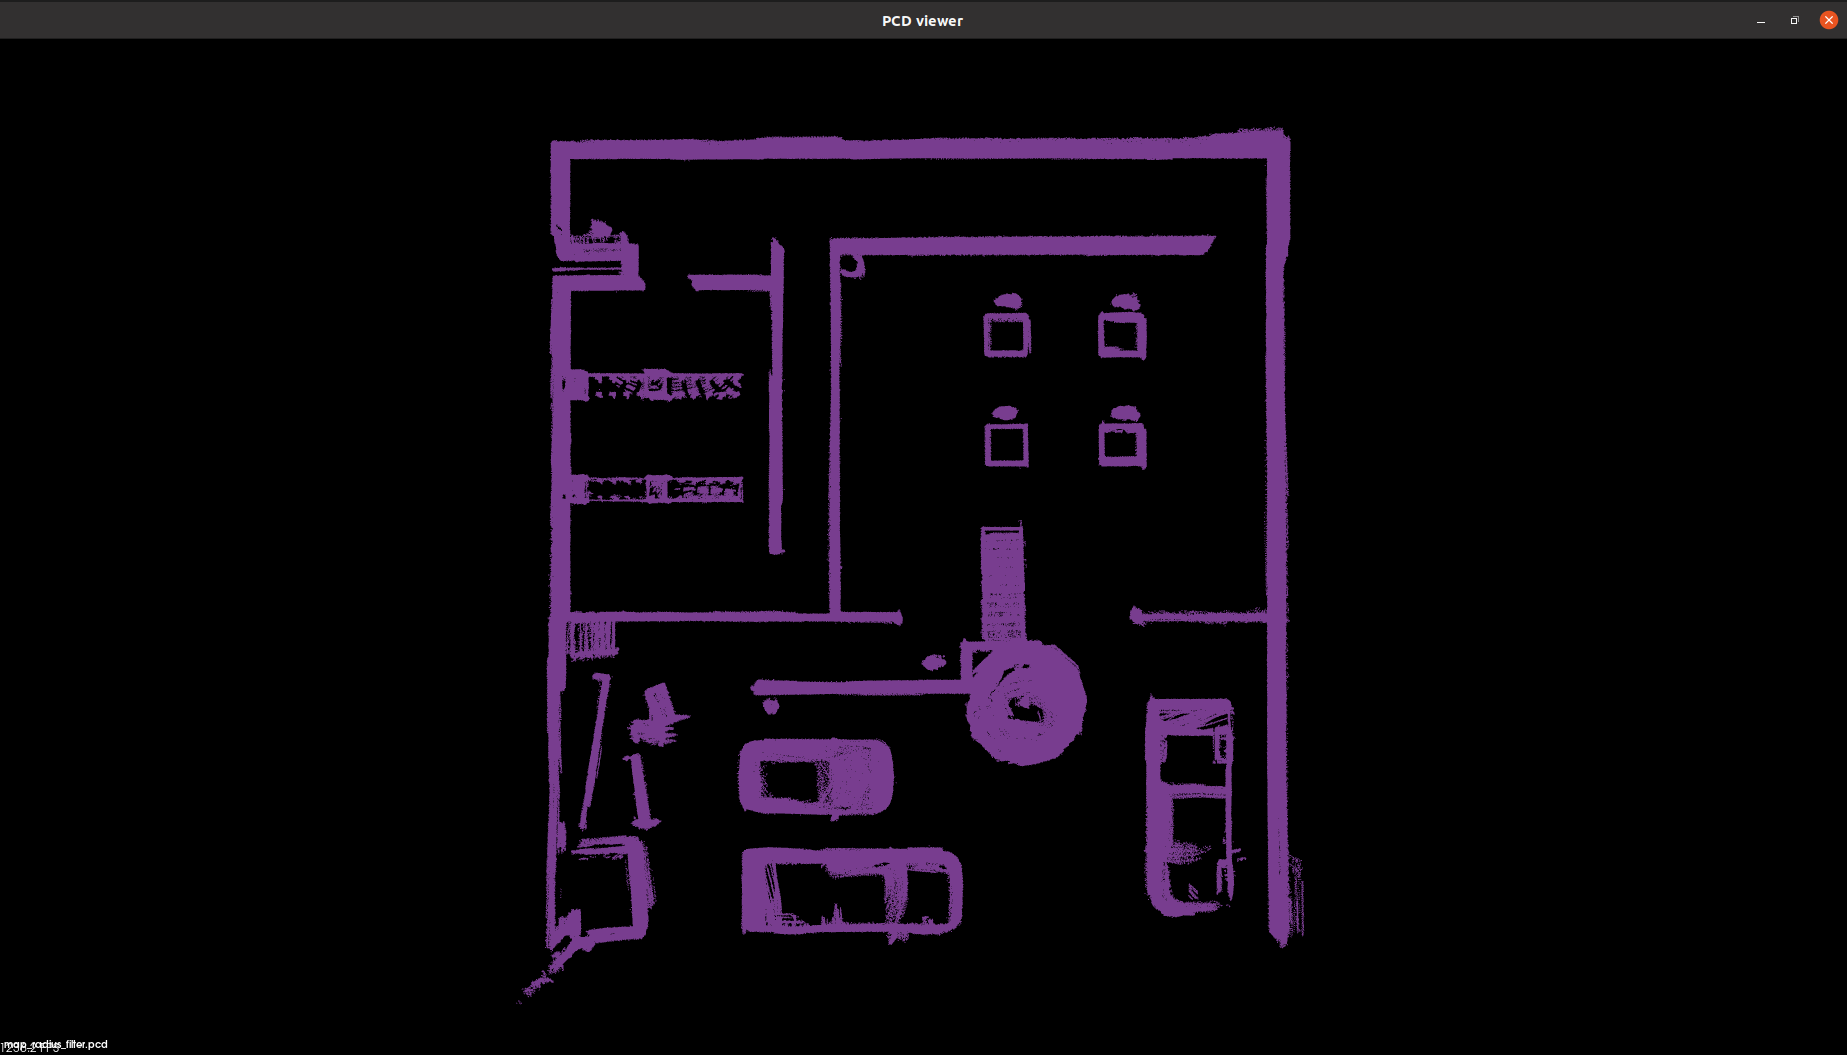
\includegraphics[width=5cm]{pcd_filtered_shot.png}
		\subcaption{Shot after filtering}
		\label{fig4b}
	\end{minipage}
	\begin{minipage}[t]{0.32\textwidth}
		\centering
		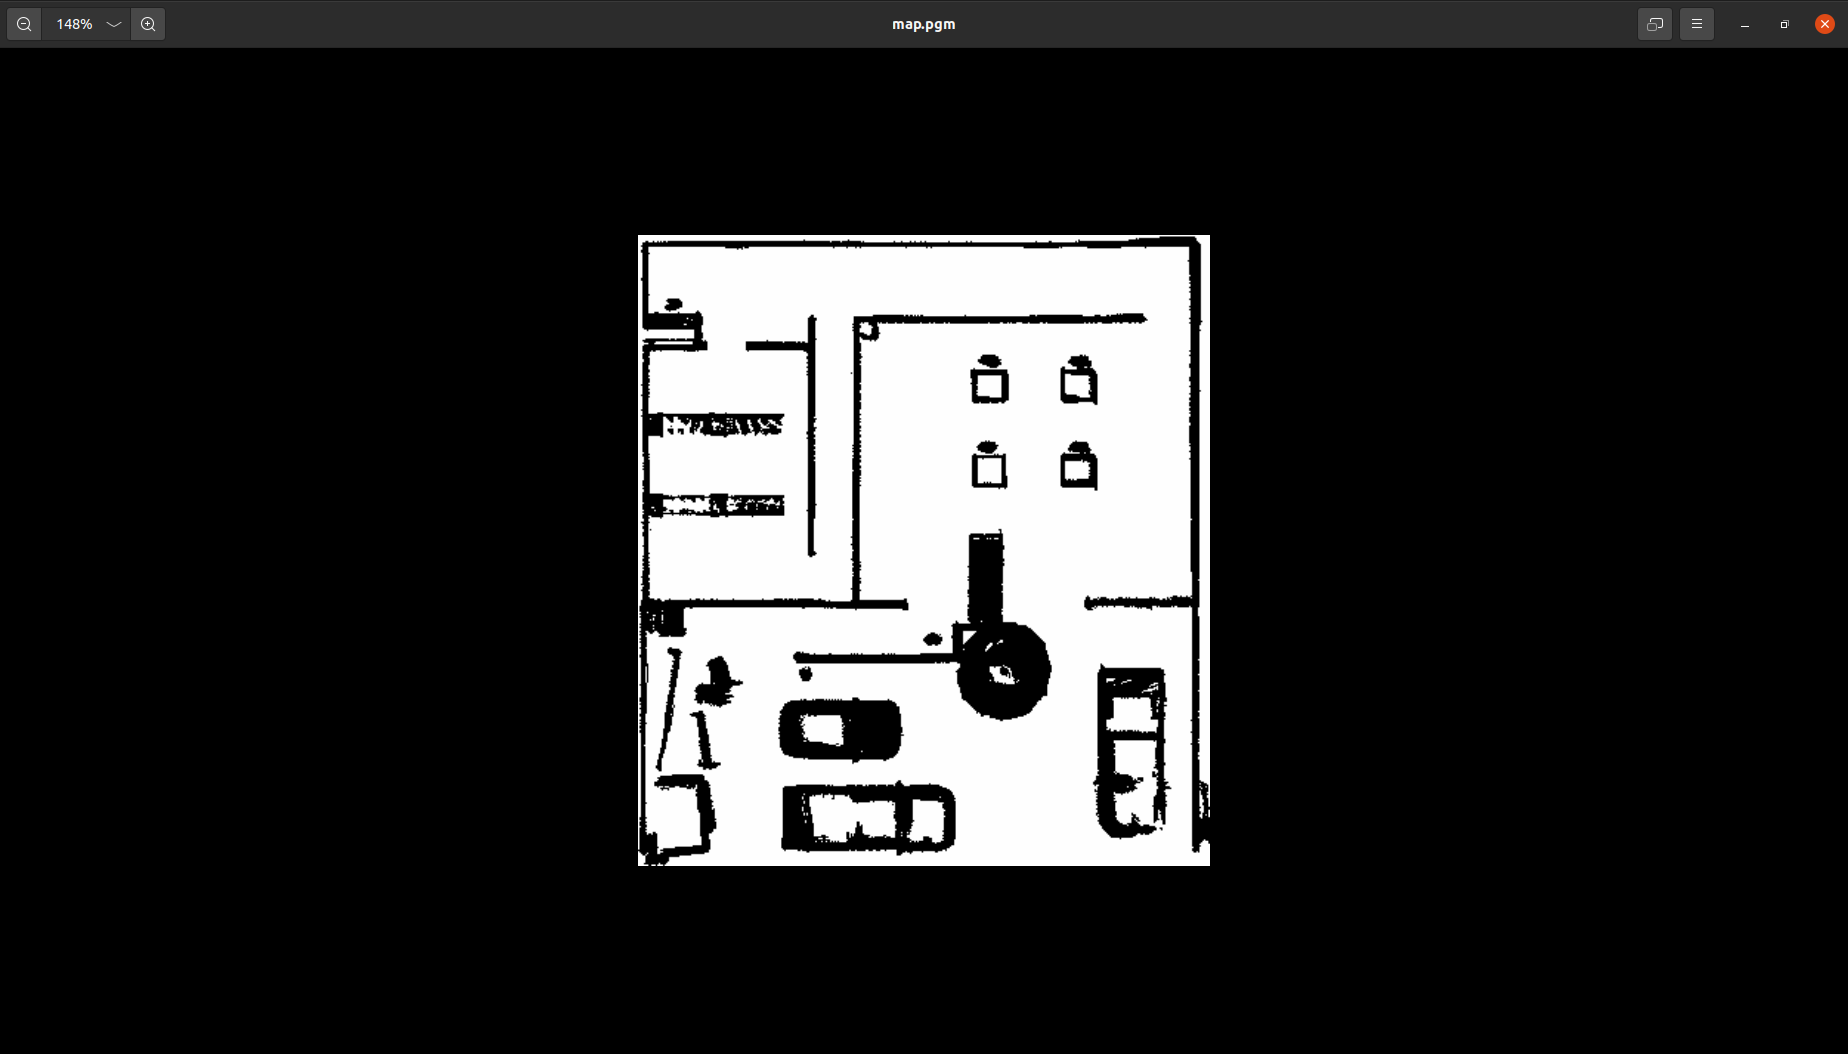
\includegraphics[width=5cm]{grid_map.png}
		\subcaption{Grid map}
		\label{fig4c}
	\end{minipage}
	\caption{Mapping results}
	\label{fig4}
\end{figure} 

\subsection{Evaluate FAST-LIO Algorithm Performance}
\hspace{1.0em}
To quantitatively evaluate the SLAM algorithm performance, here we use the method of EVO.

Here we verify the accuracy by comparing my own odometry \textit{/Odometry} topic with the published \textit{/gazebo/ground\_truth/state} topic (nav\_msgs::Odometry). The process is as follows:

\begin{itemize}[itemsep=3pt,topsep=0pt,parsep=0pt]
	\item While doing mapping, open one more terminal using command \textit{“rosbag record /gazebo/ground\_truth/state /Odometry -o EVO\_perform.bag”} to record a rosbag.
	\item Use EVO command \textit{“evo\_ape bag EVO\_perform.bag /gazebo/ground\_truth/state /Odometry -r full -va --plot --plot\_mode xy”} to evaluate and show the accuracy result.
\end{itemize}

The evaluation performance result is shown in Fig.~\ref{fig5}.

\begin{figure}[H]
	\centering
	\begin{minipage}[t]{0.45\textwidth}
		\centering
		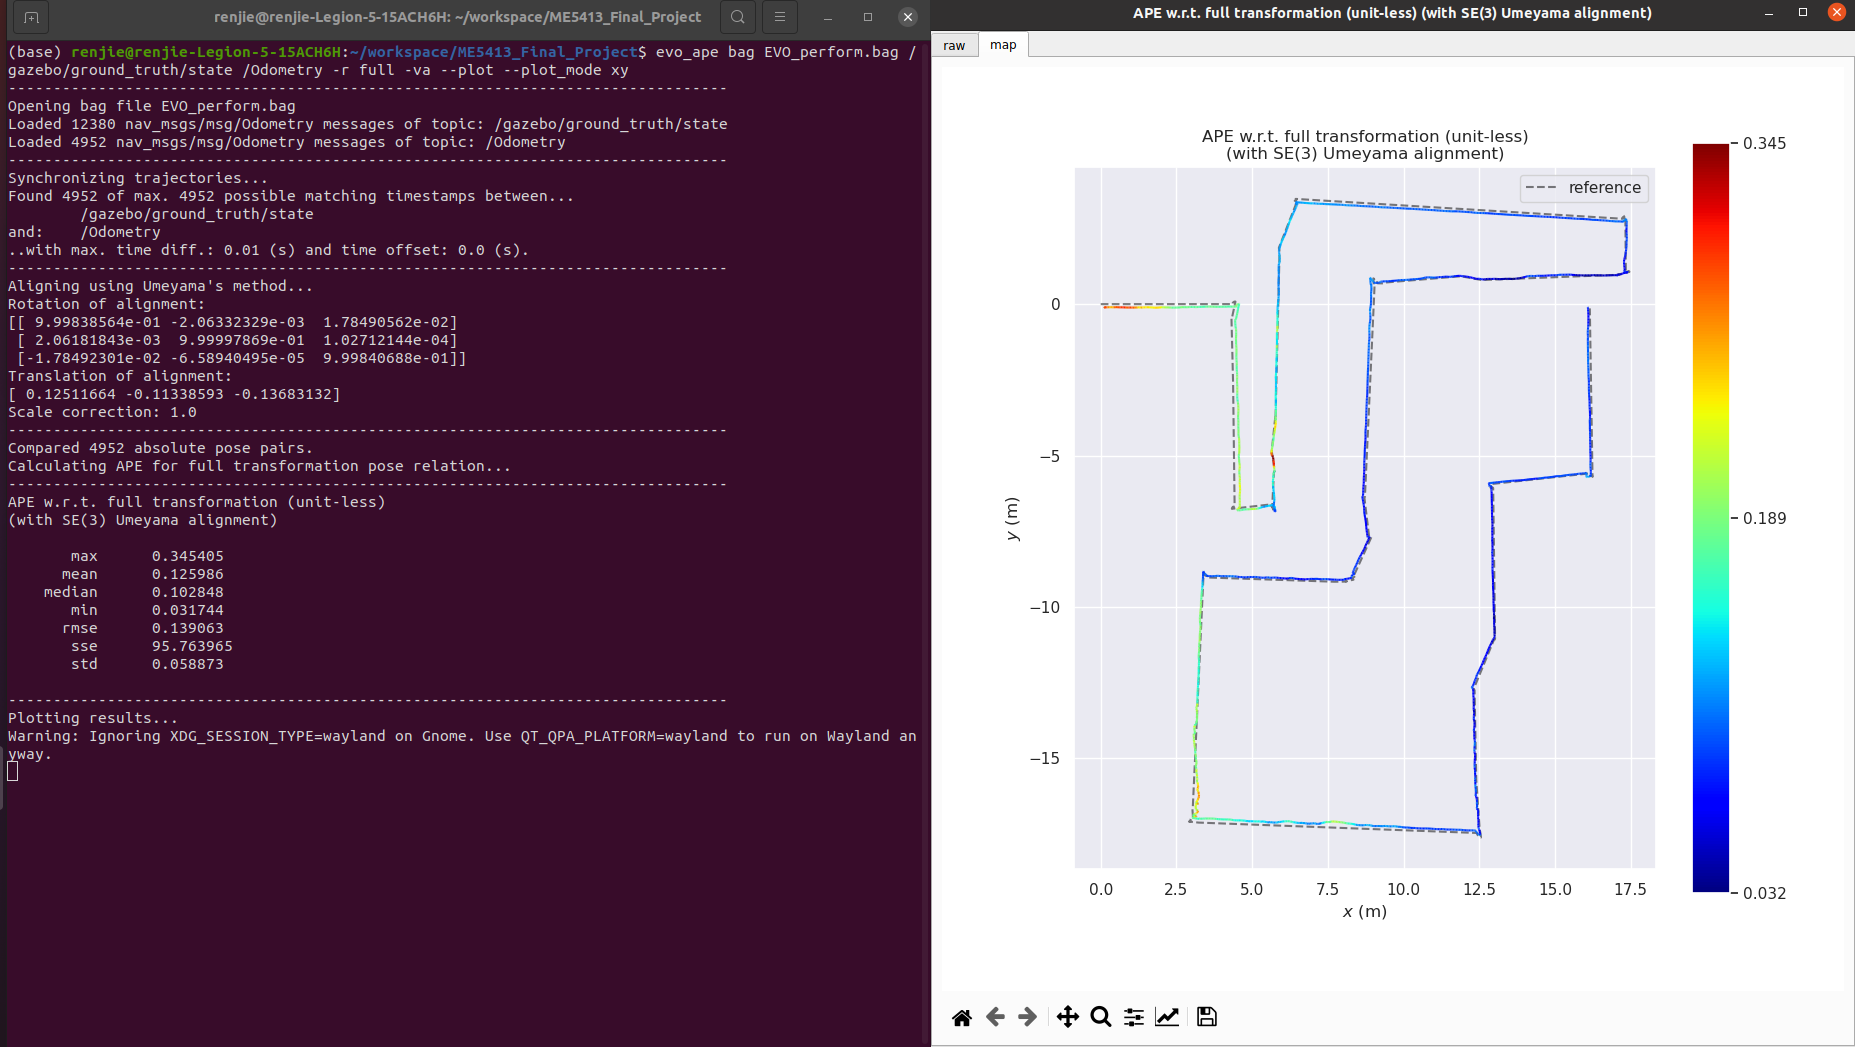
\includegraphics[width=9cm]{EVO.png}
	\end{minipage}
	\begin{minipage}[t]{0.45\textwidth}
		\centering
		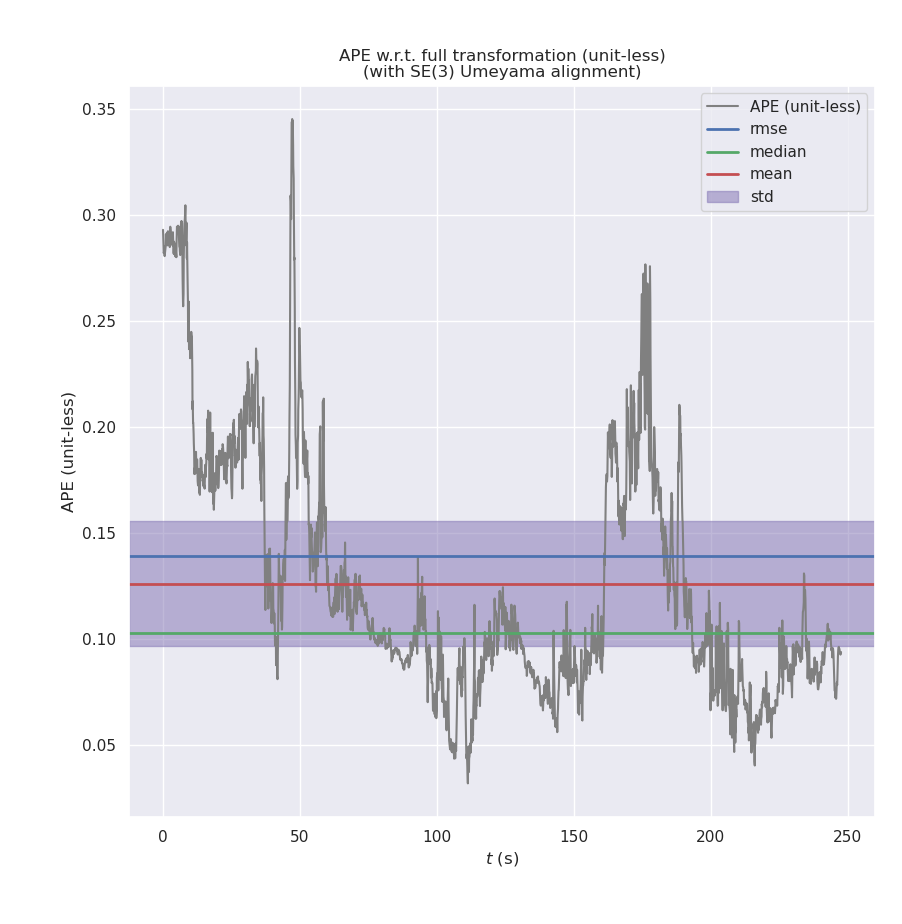
\includegraphics[width=5cm]{EVO_table.png}
	\end{minipage}
	\caption{FAST-LIO accuracy performance using EVO (figure and table)}
	\label{fig5}
\end{figure} 

As we can see from the Fig.~\ref{fig5}, the mean alignment is 0.125986 and the max alignment is 0.345405. The results show that the accuracy of algorithm performs very good.

\subsection{Discuss challenges faced and solutions}
\hspace{1.0em}
The problems that we met during doing mapping have been introduced above, which can be concluded as: 

\begin{itemize}[itemsep=3pt,topsep=0pt,parsep=0pt]
	\item[1.] Need to cut off ground cloudpoints.
	\item[2.] Fail to coincide with original cloudpoints when turning Jackal.
	\item[3.] Need to filter noise cloudpoints.
	\item[4.] Need to convert pcd file to grid map for navigation.
\end{itemize}

So, the solutions we used are:

\begin{itemize}[itemsep=3pt,topsep=0pt,parsep=0pt]
	\item[1.] Add height limit for cloudpoints in callback function and add pass-through filter to filter ground points of pcd file.
	\item[2.] Increase LiDAR rate from 10 Hz to 50 Hz.
	\item[3.] Add radius filter to remove noise points.
	\item[4.] Write algorithm package by ourselves to project pointclouds to 2D grid map.
\end{itemize}

The details could be found above in first part of Mapping Task.


\newpage

\bibliographystyle{IEEEtran}
%	
\bibliography{ref}{}

\citetext{1}{\ \ Cris.Wei (2021) FAST-LIO \ }  \href{https://github.com/nuslde/aloam_lidar_odom_result_generate}{[Source Code]}{\ \ https://github.com/hku-mars/FAST\_LIO}

\begin{appendices}
	\section{Appendix}
	
	\textbf{\textcolor[rgb]{0.98,0.00,0.00}{\textit{fast\_lio.launch}}}
	\begin{figure}[H]
		\centering
		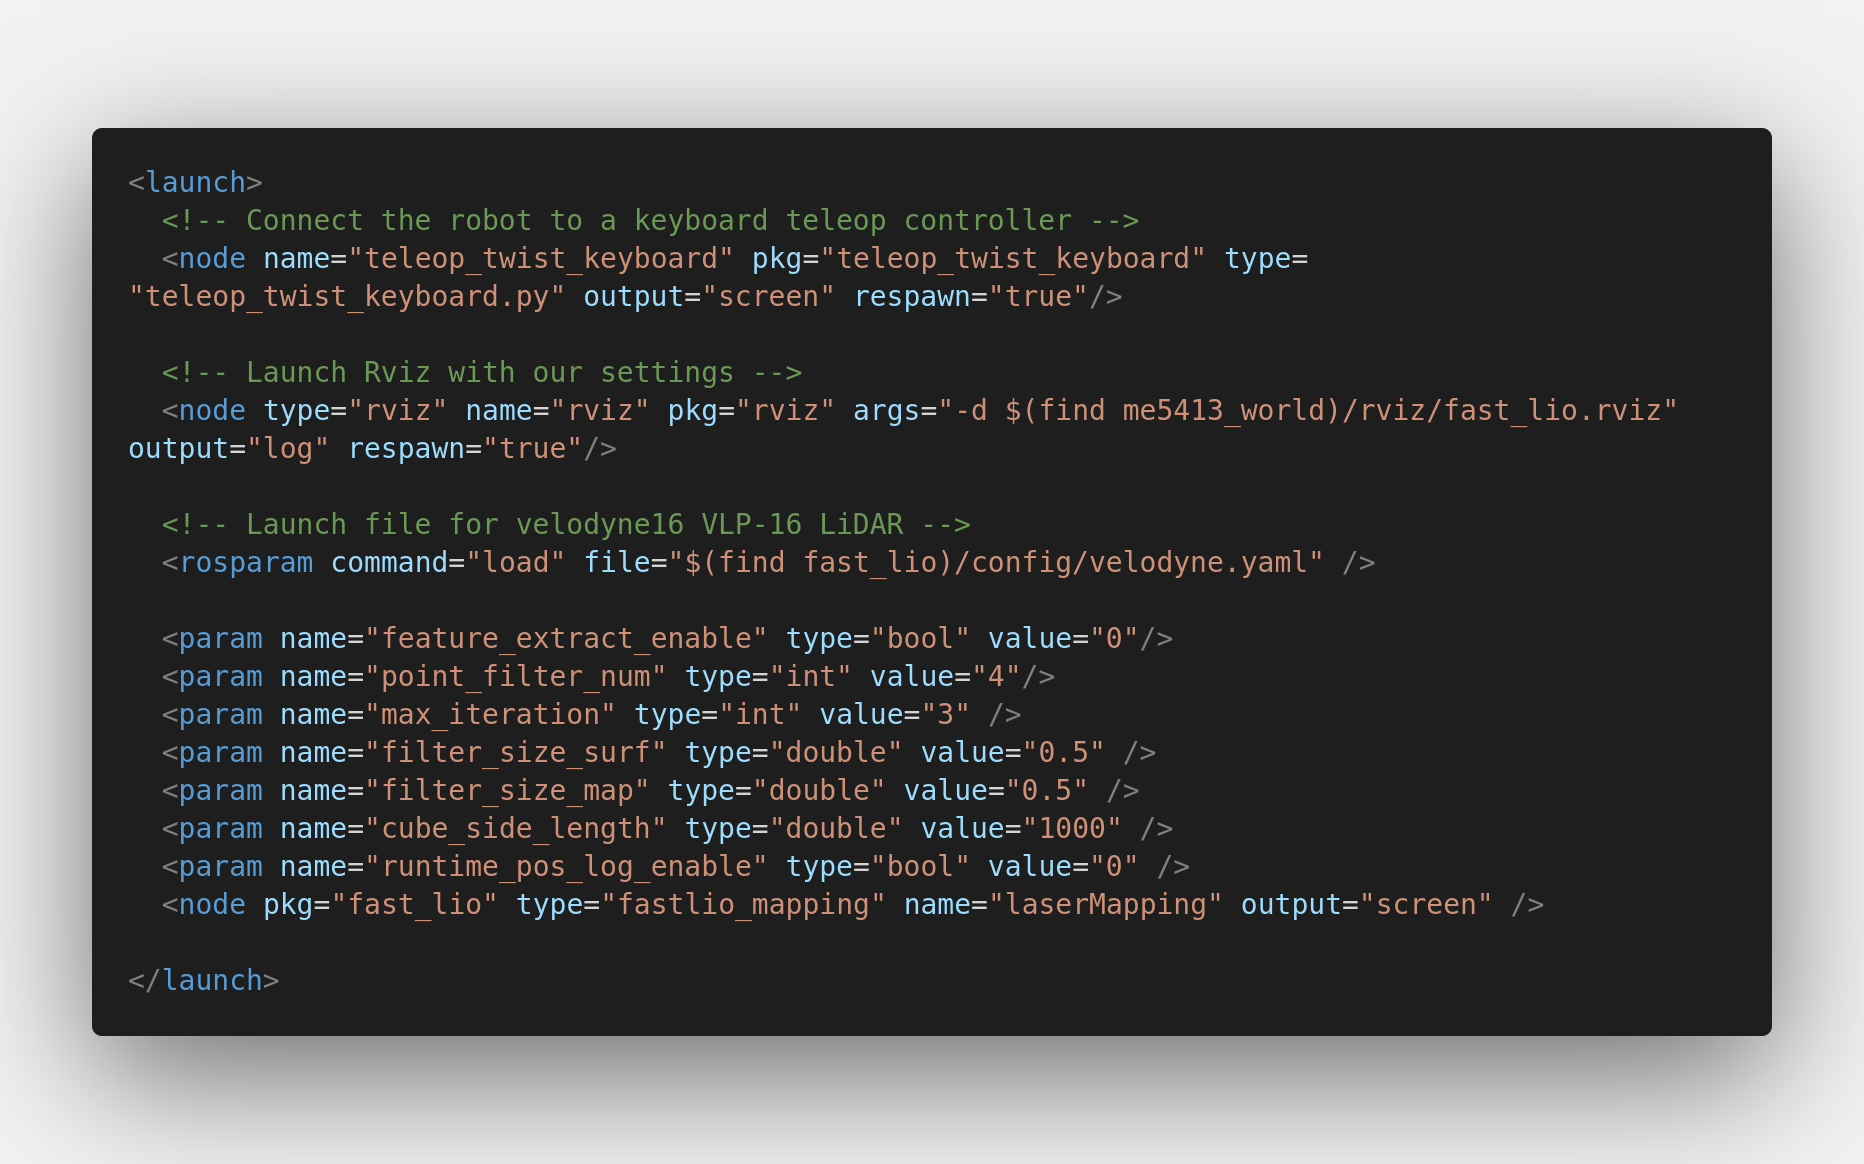
\includegraphics[width=18cm]{fast_lio_launch_code.png}
	\end{figure} 

	\textbf{\textcolor[rgb]{0.98,0.00,0.00}{\textit{velodyne.yawl}}}
	\begin{figure}[H]
		\centering
		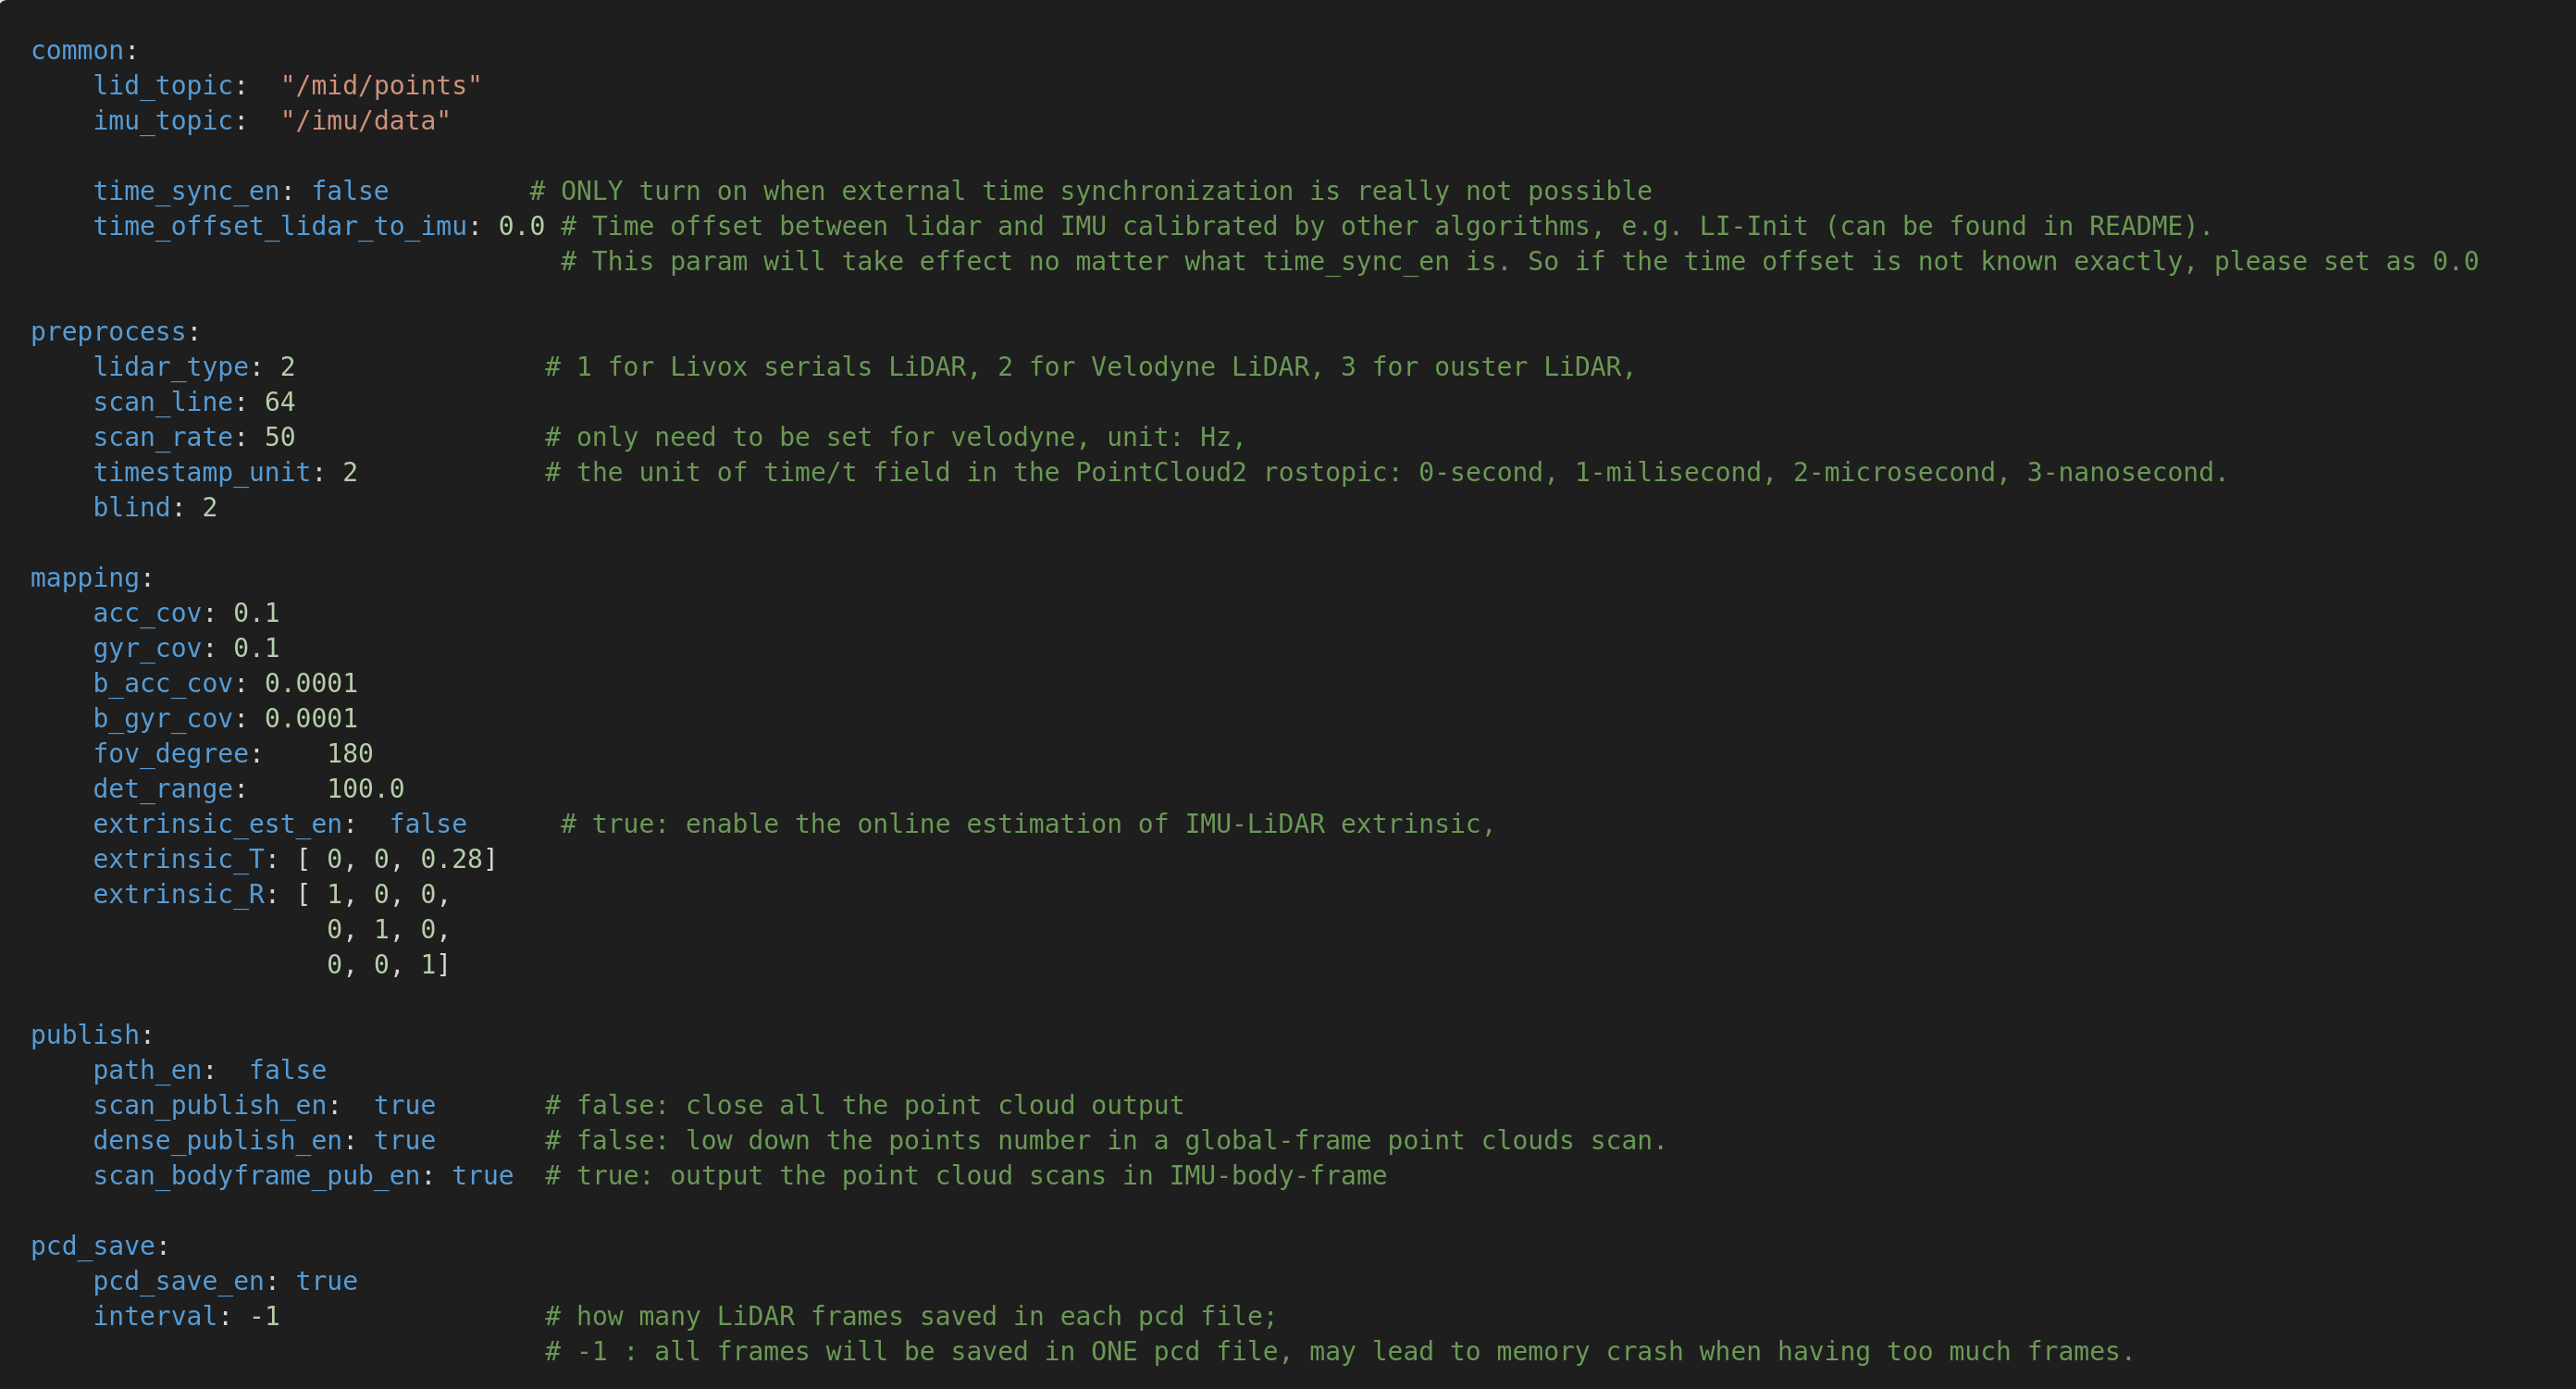
\includegraphics[width=18cm]{velodyne_config.png}
	\end{figure}

	\newpage

	\textbf{\textcolor[rgb]{0.98,0.00,0.00}{pointcloud callback function in \textit{LaserMapping.cpp}}}
	\begin{figure}[H]
		\centering
		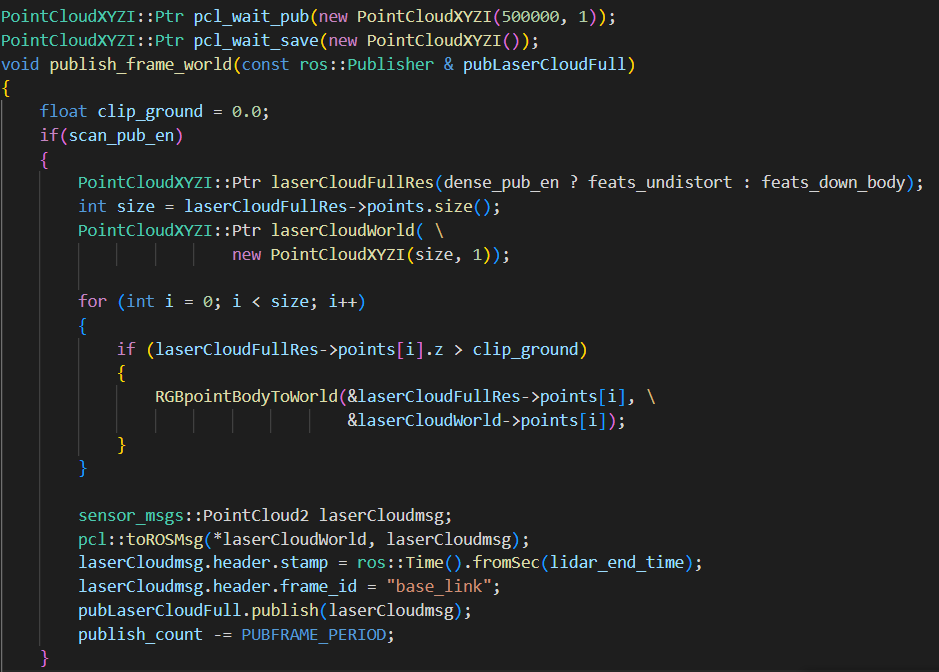
\includegraphics[width=16cm]{pointcloud_published_callback.png}
	\end{figure}

	\textbf{\textcolor[rgb]{0.98,0.00,0.00}{\textit{pcdtomap.launch}}}
	\begin{figure}[H]
		\centering
		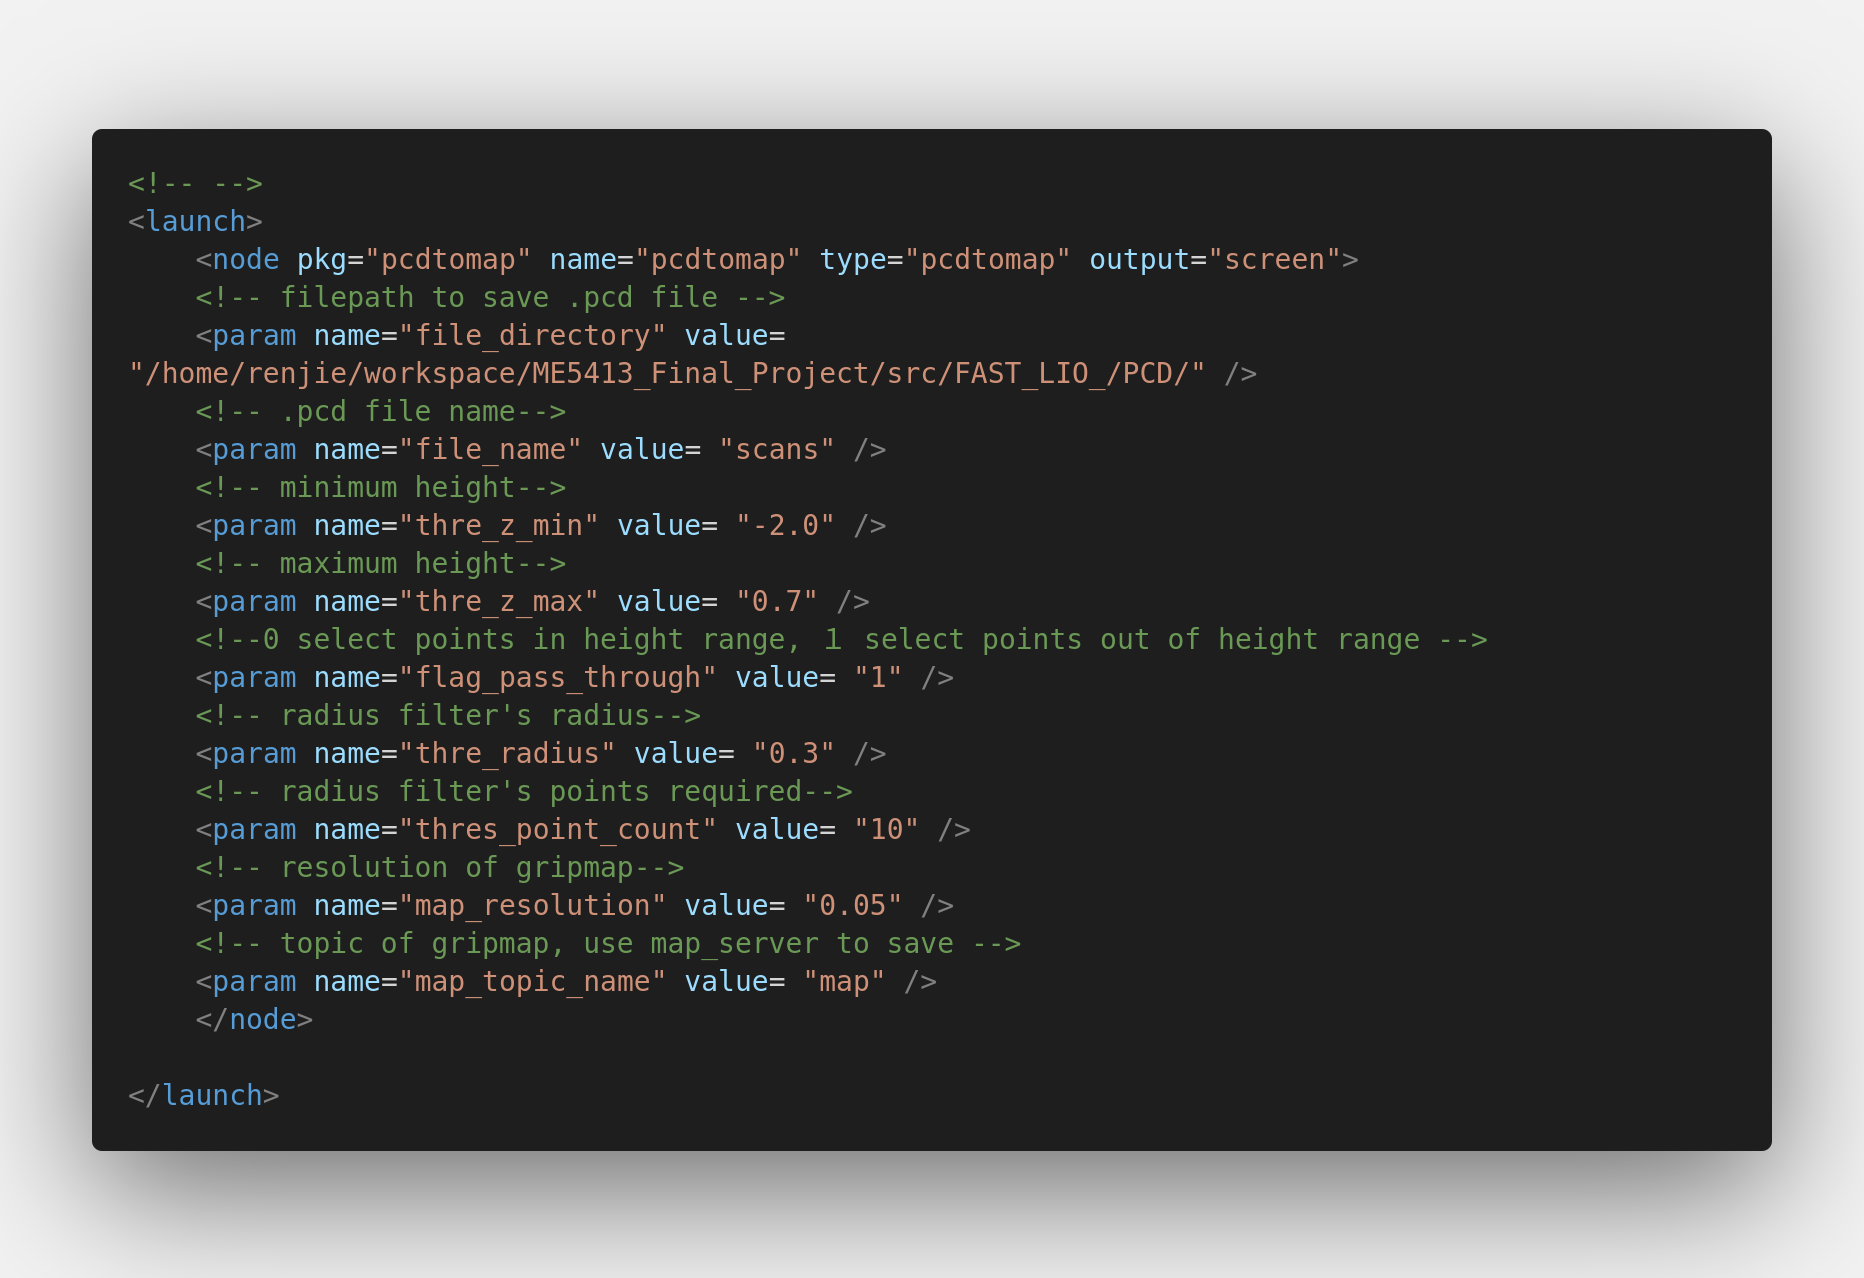
\includegraphics[width=16cm]{pcdtomap_launch_code.png}
	\end{figure}
	
\end{appendices}





	
\end{document}








